\chapter{Синтез $\mathcal{H}_\infty$-регулятора по выходу}
\label{ch:chap5}
\section{Условие задачи}

\begin{itemize}
    \item  Рассмотреть математическую модель «тележки» и для одного из наборов матриц $(C_Z,D_Z)$, выполнить следующие шаги:
    \item \item  Задаться не менее, чем двумя значениями ограничивающего параметра $\gamma > 0$.
    Постараться выбрать так, чтобы одно из этих значений было приближенным к минимальному, при котором задача еще будет иметь решение. 
    Для каждого из выбранных $\gamma$:
    \begin{itemize}
        
        \item Синтезировать соответствующий $\mathcal{H}_\infty$-регулятор вида $u = K \hat{x}$ по выходу.
        \item Синтезировать соответствующий $\mathcal{H}_\infty$-наблюдатель.
        \item Найти передаточную функцию (матрицу) Ww→z(s) замкнутой системы от внешнего возмущения $w$ к регулируемому выходу $z$.
       \item Построить для $W_{w\rightarrow z}(s)$ графики покомпонентных АЧХ.
       \item Построить для $W_{w\rightarrow z}(s)$ график сингулярных чисел.
       \item Найти $\mathcal{H}_2$ и $\mathcal{H}_\infty$ нормы  $W_{w\rightarrow z}(s)$ .
       \item Задаться не менее, чем двумя вариантами гармонического внешнего возмущения
        w на основании полученных графиков АЧХ и сингулярных чисел $W_{w\rightarrow z}(s)$. 
        Среди выбранных возмущений должен присутствовать случай, близкий к «наихудшему» и ощутимо отличающийся от него по частоте.
        \item Для каждого из выбранных вариантов внешнего возмущения $w$ выполнить моделирование и построить графики компонент регулируемого выхода $z(t)$.
        \item Сравнить полученные результаты для различных вариантов внешнего возмущения, сделать выводы.
    \end{itemize}
    \item Сравнить полученные результаты для различных вариантов ограничивающего па
    раметра $\gamma$ и сделать выводы.
\end{itemize}

\section{Решение задачи}


Теперь cинтезируем $\mathcal{H}_\infty$-регулятор по выходу, отличаться он как минимум будет тем, что \text{separation principle} в нём не выполняется
и два уравнения Риккати нужно решать вместе:
$$
\begin{cases}
    A^T \mathbf{Q} + \textbf{Q}A + C^T_Z C_Z - \textbf{Q}B(D^T_Z D_Z)^{-1} B^T \textbf{Q}  + \gamma^{-2}QB_w B^T_w \textbf{Q}= 0, \\
    K = -(D^T_Z D_Z)^{-1} B^T \textbf{Q}, \\
    A\textbf{P} + \textbf{P}A^T + B_w B_w^T - \textbf{P} C^T (D_w D_w^T)^{-1} C \textbf{P} + \gamma^{-2}\textbf{P} C^T_Z C_Z \textbf{P} = 0, \\
    L = -\textbf{P}(I - \gamma^2 \textbf{Q} \textbf{P})^{-1} (C + \gamma^{-2}D_w B_w^T \textbf{Q})^T (D_w D_w^T)^{-1}
    
\end{cases} 
$$

Помимо отсутствия \text{separation principle}, теперь нужно также проверять дополнительное условия согласованности, 
мы будем по-умолчанию при каждом синтезе проверять:
$$
    max(\sigma(PQ)) < \gamma^2
$$
% Если $B_w D_w^T = 0$, $D^T_Z D_Z$ - обратима, а также пары $(A, B_w)$ - стабилизируема, 
% $(C_Z, A)$ - обнаруживаема, то существует решение $Q > 0$ уравнения Риккати, и соответствующий наблюдатель
% имеет устойчивую динамику ошибки, также соответствующая ёй $\mathcal{H}_\infty$-норма минимальна.

\newpage
\subsection{Первый набор $(C_{Z1},D_{Z1})$}

Выберем $\gamma = 20$ и получим следующую матрицу регулятора и матрицу коррекции наблюдателя: 
$$
    K = \begin{bmatrix}
        -0.5 & -1.01 \\
    \end{bmatrix}, \tab 
    L = \begin{bmatrix}
        -1.45 \\
        -1.04 \\
    \end{bmatrix}
$$
Получим следующую передаточную матрицу системы:
$$
    W_{w\rightarrow z}(s) = \begin{bmatrix}\frac{1}{1s^{2} + 1s + 0.5} &  \frac{-2s^{3} - 3s^{2} - 2s - 0.5}{1s^{4} + 2s^{3} + 2s^{2} + 1s + 0.25} \end{bmatrix}^T
$$


\begin{figure}[ht]
    \centering
    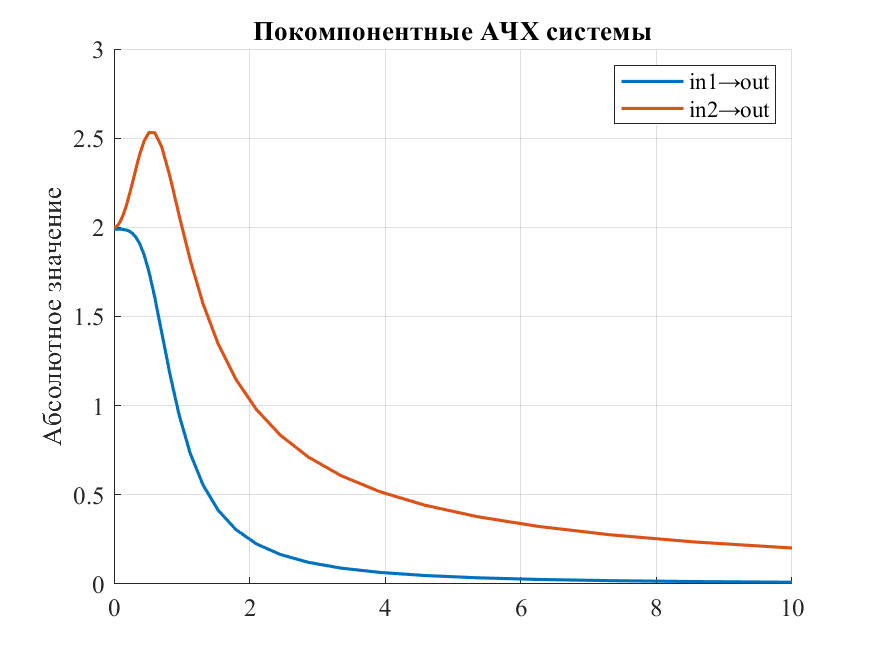
\includegraphics[width=0.8\textwidth]{freq_ampl_components9.png}
    \caption{Покомпонентные АЧХ}
  \end{figure}

\begin{figure}[ht]
  \centering
  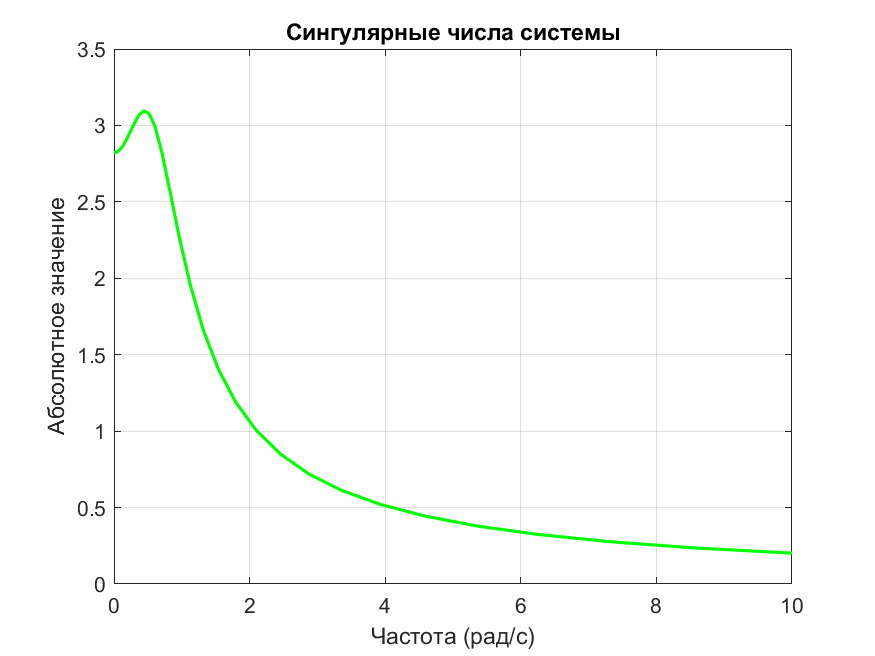
\includegraphics[width=0.8\textwidth]{singular_values9.png}
  \caption{Сингулярные числа}
\end{figure}
Нормы будем считать по следующим лекционным формулам, однако в \text{MATLAB} 
есть готовые реализации через функцию \text{norm}:
$$
    ||W||_{\mathcal{H}_2}  \approx 2.00
$$

$$
    ||W||_{\mathcal{H}_\infty}  \approx 3.09
$$

Выберем хорошую и плохую частоту $f_1, f_2$. 
Хорошей частотой для нас будет являться та, которая меньше увеличивает сигнал по амплитуде, и наоборот.
$$
    f_1 = 5.2 Hz, \tab f_2 = 0.51 Hz
$$

\subsection{Первое гармоническое возмушение}
\begin{figure}[ht]
    \centering
    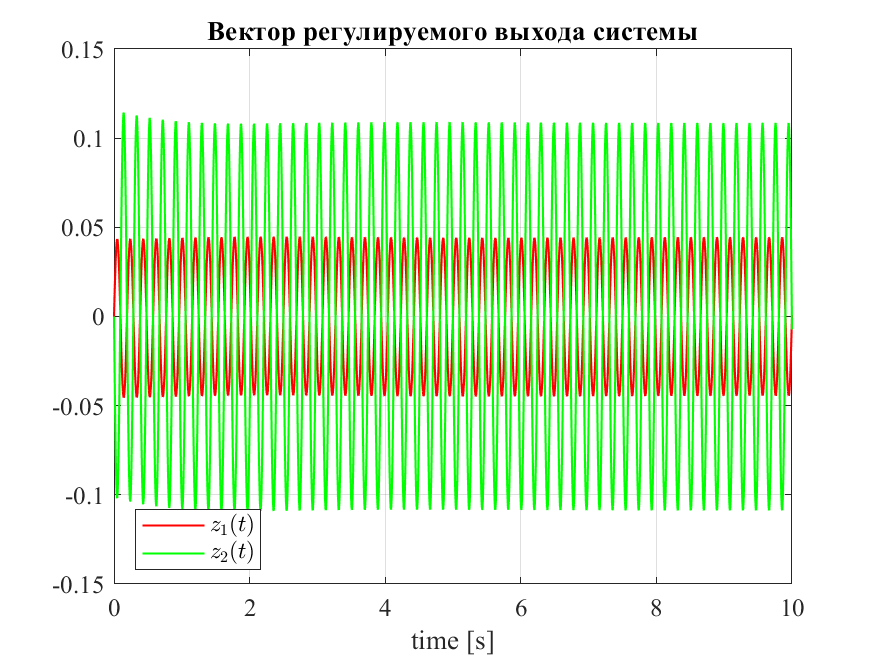
\includegraphics[width=0.8\textwidth]{z17.png}
    \caption{Моделирование -  регулируемый выход $z(t)$}
  \end{figure}

\newpage
\subsection{Второе гармоническое возмушение}
\begin{figure}[ht]
    \centering
    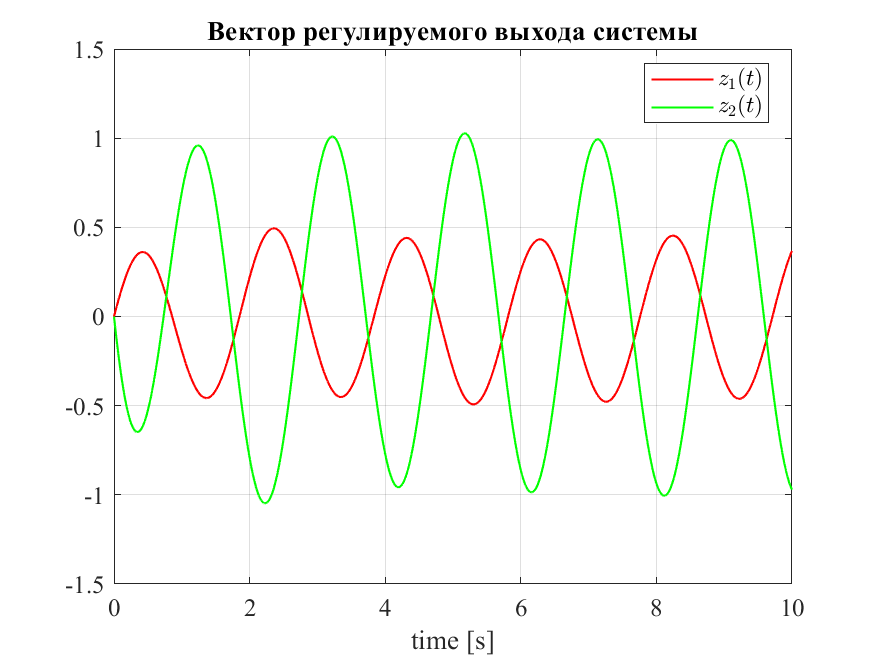
\includegraphics[width=0.8\textwidth]{z18.png}
    \caption{Моделирование -  регулируемый выход $z(t)$}
  \end{figure}


  Теперь вручную минимизируем $\gamma = 6$ и получим следующую матрицу регулятора и матрицу коррекции наблюдателя: 
  $$
      K = \begin{bmatrix}
        -0.53 & -1.09 \\
    \end{bmatrix}, \tab 
      L = \begin{bmatrix}
        -2.1 \\
        -1.71 \\
    \end{bmatrix}
  $$
  Получим следующую передаточную матрицу системы:
  $$
      W_{w\rightarrow z}(s) = \begin{bmatrix}\frac{1}{1s^{2} + 1.09s + 0.53} &  \frac{-2.18s^{3} - 3.45s^{2} - 2.32s - 0.56}{1s^{4} + 2.18s^{3} + 2.25s^{2} + 1.16s + 0.28} \end{bmatrix}^T
  $$
  
  
  \begin{figure}[ht]
      \centering
      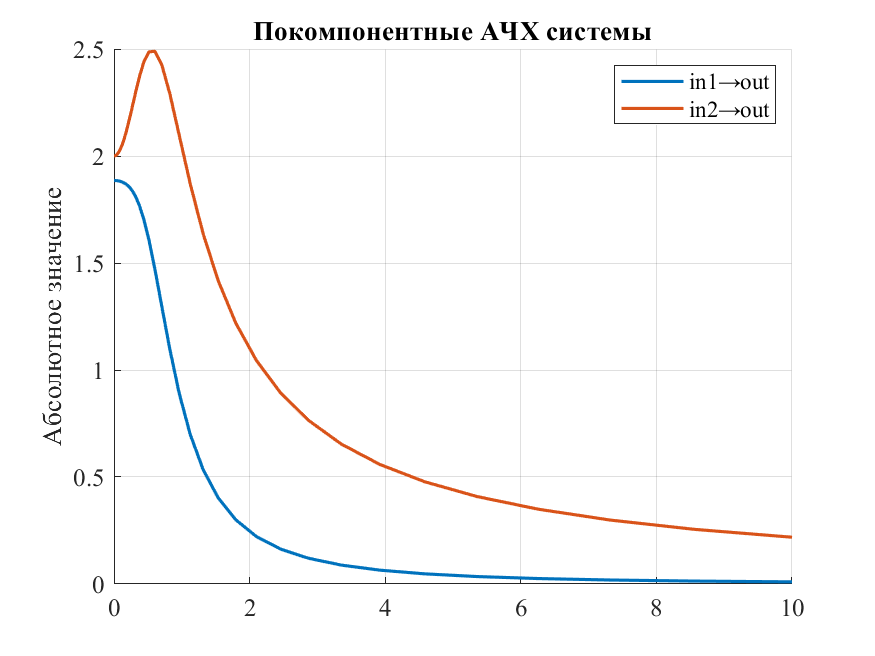
\includegraphics[width=0.8\textwidth]{freq_ampl_components10.png}
      \caption{Покомпонентные АЧХ}
    \end{figure}
  
  \begin{figure}[ht]
    \centering
    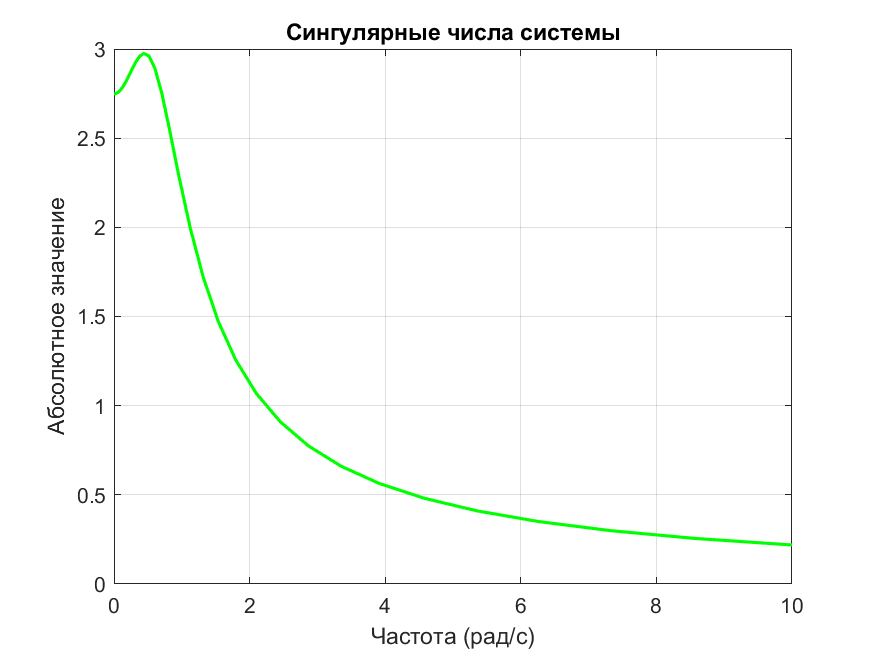
\includegraphics[width=0.8\textwidth]{singular_values10.png}
    \caption{Сингулярные числа}
  \end{figure}
  Нормы будем считать по следующим лекционным формулам, однако в \text{MATLAB} 
  есть готовые реализации через функцию \text{norm}:
  $$
      ||W||_{\mathcal{H}_2}  \approx 2
  $$
  
  $$
      ||W||_{\mathcal{H}_\infty}  \approx 2.97
  $$
  
  Выберем хорошую и плохую частоту $f_1, f_2$. 
  Хорошей частотой для нас будет являться та, которая меньше увеличивает сигнал по амплитуде, и наоборот.
  $$
      f_1 = 3.5 Hz, \tab f_2 = 0.44 Hz
  $$
  
  \subsection{Первое гармоническое возмушение}
  \begin{figure}[ht]
      \centering
      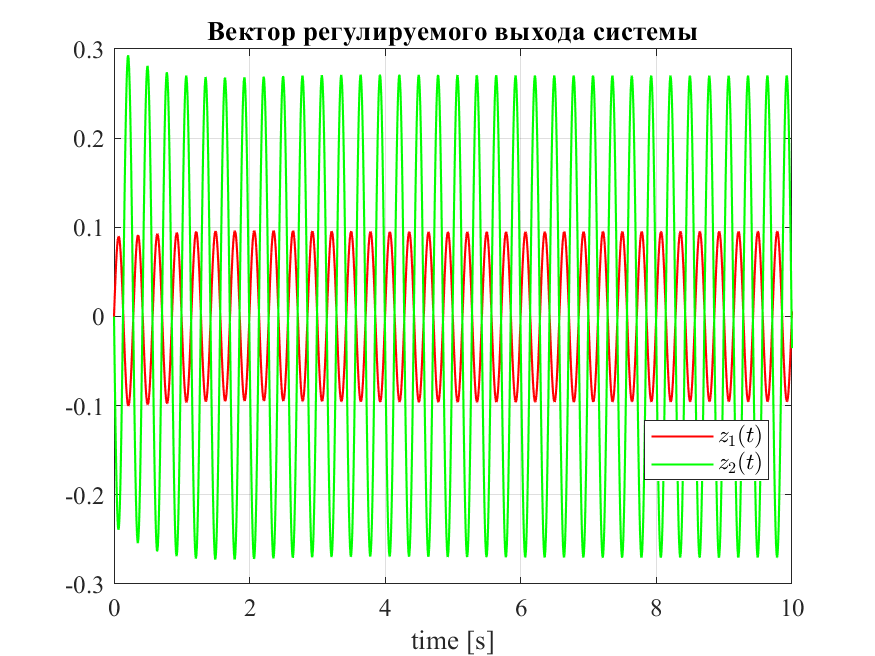
\includegraphics[width=0.8\textwidth]{z19.png}
      \caption{Моделирование -  регулируемый выход $z(t)$}
    \end{figure}
  
  \newpage
  \subsection{Второе гармоническое возмушение}
  \begin{figure}[ht]
      \centering
      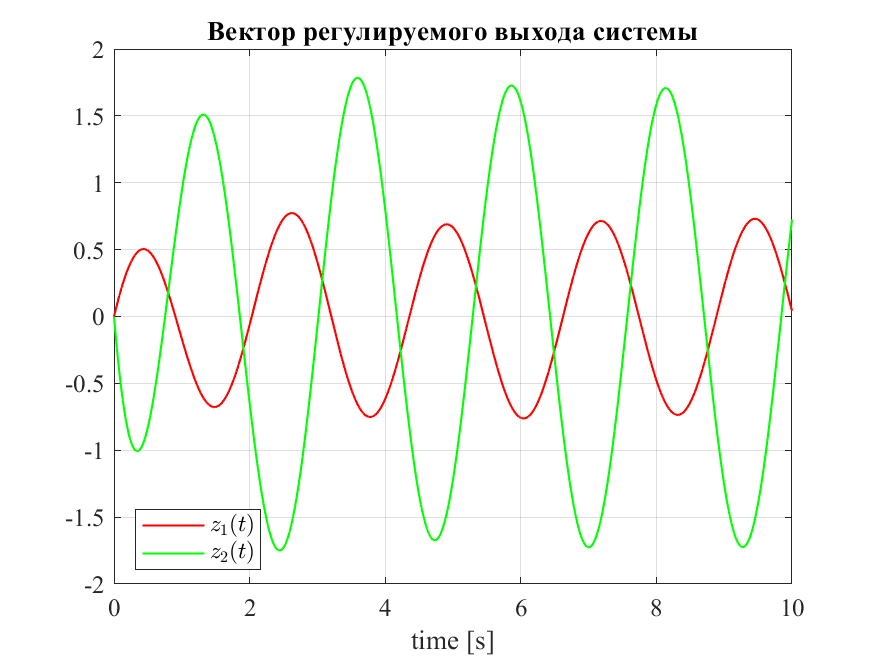
\includegraphics[width=0.8\textwidth]{z20.png}
      \caption{Моделирование -  регулируемый выход $z(t)$}
    \end{figure}
  

Амплитуда регулируемого выхода $z(t)$ различаются по своему абсолютному значению в зависимости от выбранной частоты
внешних возмущений, наблюдатель в целом показывает те же результаты, что и в прошлом задании мы получили от наблюдения непосредственно за объектом. 
При синтезе такого наблюдателя мы гарантировали $||W||_{\mathcal{H}_\infty} \leq \gamma$,  
также как и в прошлых экспериментах - пиковое сингулярное число системы действительно равняется $||W||_{\mathcal{H}_\infty}$.


\subsection{Вывод}
В этом задании мы синтезировали $\mathcal{H}_\infty$-регулятор по выходу, который нам позволил 
уменьшить значительно "приглушить" АЧХ передаточной матрицы системы в самом нежелательном месте, поэтому в результате мы получили приглушение амплитуды 
лишь в "плохих" частотах у выбранного $z(t)$.
\endinput